\section{Controlled input sensitivity}\label{sec:robustness}

These retained conditional experiments use only public decision arrays. All treatments preserve the objective form, minimum trades, holding floors and audit tolerances. Earlier scarce-ticket development results and their complete summaries remain in the replication archive.

\subsection{Input estimates and execution domains}

Twenty-four evenly spaced dates, including both endpoints of the 219-case manifest, receive target-only, covariance-only and joint shocks. Target shocks have 10/50 bp half-$L^1$ NAV distance, preserving cash and zero targets. Covariance shocks use $D\Sigma D$, $D_{ii}=\exp(\epsilon u_i)$, $u_i\in[-1,1]$, $\epsilon=0.01/0.05$, preserving positive semidefiniteness. Each runs with the original domain fixed and with optional target corridors rebuilt within unchanged full bounds. Lifecycle declarations, eligibility, group rows and cash limits stay fixed. Common preparation is repeated for rebuilt corridors. This is conditional sensitivity, not upstream estimation, changed lifecycle policy or an own-book return simulation.

All 24 baseline and 288 perturbed portfolios pass the independent audit. Risk changes are also evaluated against the original target and covariance. No case or failed output is removed.

\begin{table}[htbp]\centering\small

\caption{Large-shock allocation changes: half-$L^1$ percent of NAV.}

\begin{tabular}{llrrr}\toprule

Input & Domain & 95th pct. & Maximum & Support changed\\\midrule

Target & Fixed & 0.736 & 0.861 & 0/24\\

Target & Rebuilt & 0.803 & 0.861 & 5/24\\

Covariance & Fixed & 0.091 & 0.206 & 0/24\\

Covariance & Rebuilt & 0.091 & 0.206 & 0/24\\

Joint & Fixed & 0.669 & 0.932 & 0/24\\

Joint & Rebuilt & 0.736 & 0.932 & 5/24\\

\bottomrule\end{tabular}\end{table}

These dates overlap across treatments; they are not independent replications. The numerical archive retains turnover, common-reference risk and full weights.

\begin{figure}[htbp]\centering

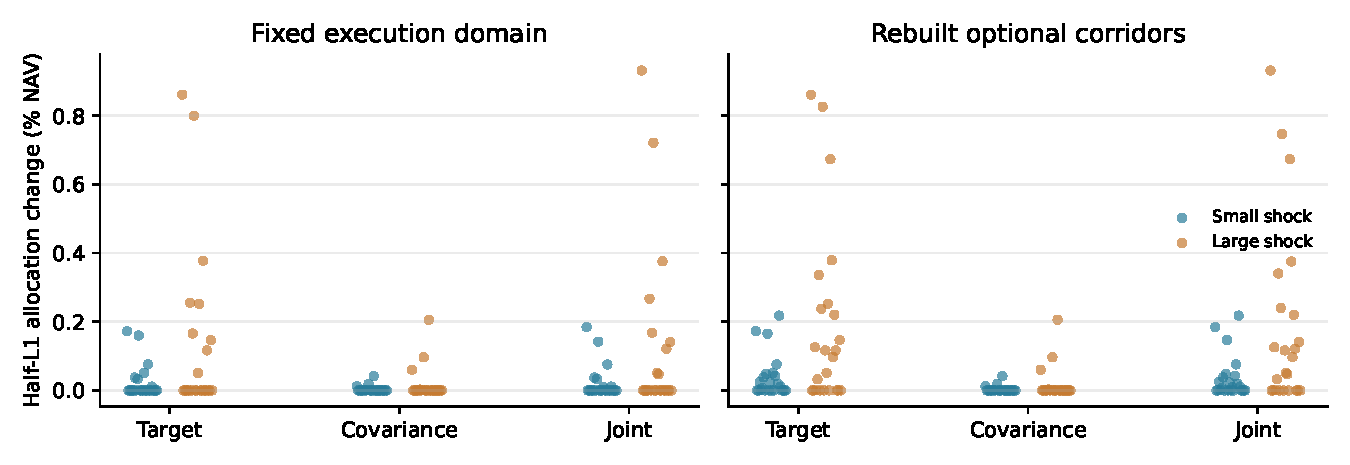
\includegraphics[width=\linewidth]{figures/sensitivity.pdf}

\caption{All conditional allocation shifts. Small/large target shocks are 10/50 NAV bp; volatility shocks have maximum absolute log shifts of 1/5 percent.}\end{figure}
